\documentclass[nojss]{jss}
%\documentclass[nojss,nofooter]{jss}
%% -- LaTeX packages and custom commands ---------------------------------------

%% recommended packages
\usepackage[plainruled,noline]{algorithm2e}
\usepackage{xcolor}
\usepackage{thumbpdf,lmodern}
\usepackage{amsmath,amssymb}
\usepackage{framed}
\usepackage{graphicx}
\usepackage{float}
\usepackage[utf8]{inputenc}
\usepackage[spanish]{babel}
\usepackage[all]{xy}

\spanishdecimal{.}

%% new custom commands
\newcommand{\class}[1]{`\code{#1}'}
\newcommand{\fct}[1]{\code{#1()}}


\SetKwInput{KwInput}{Input}  
\SetKwInput{KwOutput}{Output} 

\makeatletter
\def\@algocf@capt@plainruled{above}
\renewcommand{\algocf@caption@plainruled}{\box\algocf@capbox}%
\makeatother

\setlength\parindent{0pt} % Removes all indentation from paragraphs
\newtheorem{Def}{Definition}
\newtheorem{prop}{Proposition}
\newtheorem{eje}{Example}
\newtheorem{teo}{Theorem}
\newtheorem{lem}{Lemma}
\newtheorem{cor}[teo]{Corolarie}
\newtheorem{Obs}{Observation}


\def \dem{\paragraph{Demostración\\}}
\def \enddem{ \hfill $\blacksquare$}

%% -- Article metainformation (author, title, ...) -----------------------------

\author{Izhar Asael Alonzo Matamoros \\  Universidad de Cantabria \\}
\Plainauthor{Izhar Asael Alonzo Matamoros}


\title{\huge Redes neuronales Bayesianas para regresión}
\Plaintitle{Redes neuronales Bayesianas para regresión}
\Shorttitle{Redes neuronales Bayesianas para regresión}

\Abstract{En este trabajo se da una introducción a las redes neuronales Bayesianas para resolver problemas de regresión, se discute su complejidad y problemas de identificabilidad, es decir, la imposibilidad de obtener un buen ajuste de los parámetros desconocidos. Además, se presentan las redes como un modelo de regresión y se proveen referencias de sus relaciones con otros modelos. Finalmente, se realiza un caso de estudio para mostrar sus problemas de identificabilidad y su alto poder predictivo.}

\Keywords{Redes Neuronales, regresión, modelos lineales, Inferencia Bayesiana}
\Plainkeywords{Redes Neuronales, regresión, modelos lineales, Inferencia Bayesiana}

\Address{
  Izhar Asael Alonzo Matamoros\\
  Universidad Nacional Autónoma de Honduras\\
  Departmento de Estadística\\
  Escuela de Matemática, Facultad de Ciencias\\
  Blvd Suyapa, Universidad Nacional Autónoma de Honduras\\
  Tegucigalpa, Honduras\\
  E-mail: \email{asael.alonzo@gmail.com}\\
  URL: \url{https://asaelam.wixsite.com/asael697site}
}

\begin{document}



\section{Introducción}
Este trabajo es una breve introducción de las redes neuronales Bayesianas, y se presentan como una generalización del problema de regresión. De igual forma, son equivalentes a una aproximación polinómica y convergen asintóticamente a un proceso gaussiano. Además, se introduce el problema de identificación que las redes poseen debido a la sobre-parametrización y complejidad, presentando también algunas referencias que han podido lidiar con dicha problemática.\\

Como caso de estudio, se analiza los precios de casas, de la data Housing. Se implementa una red neuronal Bayesiana con una capa escondida, con 4 neuronas y prioris independientes, y se compara con una regresión lineal Bayesiana con prioris multivariadas para modelar la dependencia de los parámetros. Pese los altos costos computacionales, la mala interpretación de los modelos, y la no identificabilidad de los parámetros, la red neuronal ofrece mejores predicciones frente a la regresión lineal.\\

El trabajo de divide de la siguiente forma, en la \textit{sección 2} se introducen las redes neuronales, y su representación gráfica. En la \textit{sección 3}, se define una red neuronal como modelo de regresión, se presenta el modelo lineal como caso particular de una red neuronal, y se discute de sus equivalencias con otros modelos. En la \textit{sección 4}, se introducen las redes neuronales Bayesianas y se presenta la ecuación de actualización de Bayes para estos modelos. En la \textit{sección 5}, se realiza un análisis de los datos usando modelos lineales y redes neuronales, se da un breve resumen de la inferencia de los parámetros y convergencia de los mismos. Finalmente, en la \textit{sección 6}, se da una comparación del ajuste y predicciones de ambos modelos.
  
\section{Redes Neuronales}

Las redes neuronales (NN) son funciones no lineales $NN:\mathbb{R}^n \rightarrow \mathbb{R}^m$, que en principio, pueden modelar cualquier mapeo \textit{suave} de  $\mathbb{R}^n$ a $\mathbb{R}^m$. A las variables predictivas de la red se les conoce como entradas (\textit{inputs}) y a las  dependientes se les conoce como salida (\textit{output}). Una NN puede ser vista como un conjunto neuronas organizadas en capas (\textit{layers}), las variables predictivas forman la primera capa, las dependientes la  última, y las capas intermedias (\textit{Hidden Layers}) contienen a las neuronas \cite{Paige2001}. La dinámica de una red neuronal puede ser representada mediante un diagrama, en la \textit{figura 1} se muestra una red neuronal con 5 variables predictivas (\textit{columna Entradas}), 2 capas ocultas con 3 neuronas cada una, y una variable dependiente (\textit{columna salidas}).

\begin{figure}[H]
\centering
$$
\xymatrix{
	\text{Entradas}                     &  \text{Capa 1}                   & \text{Capa 2}      &\text{Salidas}\\
	*+[o][F]{E1}\ar[dr]\ar[ddr]\ar[dddr]&                                  &                    & \\
	*+[o][F]{E2}\ar[r] \ar[dr] \ar[ddr] &*+[o][F]{C11}\ar[r]\ar[dr]\ar[ddr]&*+[o][F]{C12}\ar[dr]& \\
	*+[o][F]{E3}\ar[dr]\ar[ur] \ar[r]   &*+[o][F]{C21}\ar[r]\ar[ur]\ar[dr] &*+[o][F]{C22}\ar[r] & *+[o][F]{S}\\
	*+[o][F]{E4}\ar[r] \ar[ur] \ar[uur] &*+[o][F]{C31}\ar[ur]\ar[r]\ar[uur]&*+[o][F]{C32}\ar[ur]& \\	
	*+[o][F]{E5}\ar[ur]\ar[uur]\ar[uuur]&                                  &                    & \\		
}
$$
\caption[Red Neuronal]{Red Neuronal con dos capas ocultas}
\label{fig:fig1}
\end{figure}

La interacción neuronal de las redes se modela con correspondencias no lineales, que se les denota como la función de activación ($\phi$), las más populares son: la función logística (\textit{sigmuid}), y la  tangente hiperbólica (\textit{tanh}), \cite{Bhat2006}. Las Redes Neuronales pese que son simples modelos para simular la dinámica cerebral, son poderosos modelos predictivos que han sido de gran utilidad en el análisis de datos, para tratar problemas de clasificación y regresión. Pese a su alto poder predictivo, las NN sufren de poca interpretación sobre el fenómeno físico,  sobre parametrización (\textit{alta cantidad de parámetros}), no identificabilidad (\textit{múltiples soluciones óptimas locales}), y mala aproximación en la inferencia de los parámetros (poca convergencia de los algoritmos de optimización y posterioris multimodales) dificultando el aprendizaje estadístico y automatizado, para un mayor contexto teórico revisar \cite{tensorflow2015} o \cite{haykin2009}. 

\section{Regresión}

Este trabajo se enfoca en el problema de regresión, este consiste en estimar la curva que mejor explica la relación entre la variable dependiente Y (\textit{salida}) y un conjunto de variables explicativas X (\textit{entradas}). El problema de regresión puede ser escrito de la siguiente forma:

\begin{Def}
	Sea $Y = \{Y_1,Y_2,\ldots,Y_n\}$ un conjunto en $\mathbb{R}$ que representa una muestra aleatoria de la variable dependiente Y, y sea $X = \{X_1,X_2,\ldots,X_n\}$ un conjunto en $\mathbb{R}^d$ que representa una muestra aleatoria de variables explicativas X. Entonces, el problema de regresión consiste en estimar el funcional $f:\mathbb{R}^d \rightarrow \mathbb{R}$ tal que:
	$$Y_i = f(X_i) +\epsilon_i$$
	Donde $\epsilon_i \sim N(0,\sigma^2)$ representa un ruido blanco Gaussiano centrado en 0.
\end{Def}

Los modelos más utilizados para  el problema de regresión son los modelos lineales, que consisten en asumir que el funcional $f$ es lineal ($f(X) = aX +b$). Estos modelos poseen supuestos muy fuertes (\textit{no colinealidad y homogeneidad)} y generalmente ofrecen pobres predicciones. Los modelos lineales son un caso particular de las redes neuronales (\textit{NN sin capas ocultas}), en la \textit{figura 2} se presenta el diagrama de un modelo lineal visto como una red neuronal.


\begin{figure}[H]
 \centering
 $$
 \xymatrix{
  \text{Entradas}     &\text{Salidas}\\
  *+[o][F]{E1}\ar[ddr]& \\
  *+[o][F]{E2}\ar[dr] & \\
  *+[o][F]{E3}\ar[r]  & *+[o][F]{S}\\
  *+[o][F]{E4}\ar[ur] & \\	
  *+[o][F]{E5}\ar[uur]& \\		
 }
 $$
 \caption[Modelo lineal]{Diagrama de un modelo lineal}
 \label{fig:fig2}
\end{figure}
 
\begin{Def}
	Sea $Y = \{Y_1,Y_2,\ldots,Y_n\}$ una muestra aleatoria en $\mathbb{R}$ para la variable dependiente Y, y sea $X = \{X_1,X_2,\ldots,X_n\}$ una muestra aleatoria en $\mathbb{R}^d$ de las variables explicativas X. Se dicen que X e Y siguen un modelo lineal si existe un vector de parámetros $\theta = (\beta_0,\beta_1, \ldots,\beta_d) \in\Theta = \mathbb{R}^{d+1}$ tal que se satisface la siguiente ecuación.
	$$Y_i = \beta_0 + \sum_{i=1}^d \beta_i X_i +\epsilon_i$$
	Donde $f(X) = \sum_{i=1}^d\beta_iX_i$ es el funcional asociado al problema de regresión y $\epsilon_i \sim N(0,\sigma^2)$ es un ruido blanco Gaussiano centrado en 0.
\end{Def}
 
 
A diferencia de las NN, los modelos lineales ofrecen simplicidad de interpretación, implementación con bajo costo computacional, e identificabilidad (\textit{solución óptima global}). Estos modelos son utilizados previo a la implementación de una red neuronal para identificar las variables predictoras que mayor explican a la variable dependiente, y para la identificación de variables colineales.\footnote{Dos variables $X_1$ y $X_2$ se dicen colineales, si existe una relación lineal g tal que $X_1 = g(X_2)$.}

\begin{Def}
	Sea
	\begin{itemize}
		\item $Y = \{Y_1,Y_2,\ldots,Y_n\}$ una muestra aleatoria en $\mathbb{R}$ para la variable dependiente Y.
		\item $X = \{X_1,X_2,\ldots,X_n\}$ una muestra aleatoria en $\mathbb{R}^d$ de las variables explicativas X.
		\item  c el número de capas ocultas de la red neuronal.
		\item $h_i,\text{ } i = 1,2,\ldots c$ el número de neuronas  en la i-ésima capa de la red.
		\item $Z_j = \{Z_{j1},Z_{j2},\ldots, Z_{jh_i}\}$ la colección de neuronas en la i-ésima capa.
		\item $\phi$ la función de activación de las neuronas
	\end{itemize}
	 
	Se dicen que X e Y siguen un modelo de redes neuronales multicapas, si existe una colección de parámetros $\theta = \left\{ \{\beta_i\}_{i=0}^{c},\{\alpha_{0,i}\}_{i=0}^{d},\{\alpha_{1,i}\}_{i=0}^{h_1},\ldots, \{\alpha_{c,i}\}_{i=0}^{h_c}, \right\} \in \Theta$ tal que se satisface la siguiente ecuación recursiva.
	$$Y_i = \beta_{0} + \sum_{k=1}^{h_c} \alpha_{h_c,k} Z_c +\epsilon_i, \text{ } i = 1,2,\ldots,n$$
	Donde: 
	$$Z_{j} = \phi\left(\beta_j +\sum_{k=1}^{h_j}\alpha_{j-1,k}Z_{k,j-1}\right)\text{ } j = 1,2,\ldots,c$$
	y 
	$$Z_{1} = \phi\left(\beta_1 +\sum_{k=1}^{d}\alpha_{0,k}X_{k}\right) $$
	
	Donde$f(Z) = \sum_{k=1}^{h_c} \alpha_{h_c,k} Z_c$ es el funcional asociado al problema de regresión, y  $\epsilon_i \sim N(0,\sigma^2)$ es un ruido blanco Gaussiano centrado en 0.
\end{Def}

Estimar $f$ en una red neuronal es un problema muy complicado, posee un alto costo computacional, y sufre problemas de identificabilidad, que en parte ocurren por la no-linealidad y sobreparametrización del modelo, resultando en muchas soluciones equivalentes. Existen muchas alternativas para resolver parcialmente esta problemática, como implementar los algoritmos en varios puntos iniciales aleatorios para evitar soluciones en mínimos locales, reducir la dimensión de X (\textit{componentes principales}), reparametrización del modelo inicial, \cite{Arya2017}.\\

Existen otras alternativas a las redes neuronales que ofrecen resultados aceptables y con mayor facilidad de interpretación y sin problemas de identificabilidad, como los modelos aditivos generalizados \cite{Rigby2005}, regresión con penalización, splines \cite{Silverman1985}, y procesos gaussianos \cite{gramacy2020surrogates}.  
 
\section{Redes neuronales Bayesianas} 
 
 Una red neuronal Bayesiana es un modelo NN donde se asume que los parámetros desconocidos $$\theta = \left\{ \{\beta_i\}_{i=0}^{c},\{\alpha_{0,i}\}_{i=0}^{d},\{\alpha_{1,i}\}_{i=0}^{h_1},\ldots, \{\alpha_{c,i}\}_{i=0}^{h_c}, \right\} \in \Theta$$ 
Son variables aleatorias, de los cuales se conoce su información a priori, resumida en una función de probabilidad $P(\theta)$ \cite{Bhat2006}. Por lo tanto, se desea conocer la función de probabilidad de $\theta$ dado los valores de la muestra $P(\theta/Y)$ mediante el teorema de actualización de Bayes. \cite{Miggon} y \cite{degroot19886}\\

Usando la \textit{definición 3}, la muestra para la variable de salida Y puede ser reescrita de la forma:
$$Y \sim N(f(Z/\theta),\sigma^2)$$
Donde $f(Z/ \theta)$ es el funcional asociado al modelos NN condicionado al conjunto de parámetros. Por lo tanto, la función de verosimilitud es simplemente el producto de las marginales
$$P(Y/\theta) = \prod_{i=1}^n\dfrac{1}{\sqrt{2\pi\sigma^2}}exp \left\{ - \dfrac{(Y_i- f(Z_i/\theta) )^2}{2\sigma^2} \right\}$$
Las distribuciones a priori de cada uno de los parámetros se asumen independientes entre si, por lo tanto, P se escribe de la forma:
 $$P(\theta) = P(\sigma^2)\prod_{k=1}^cP(\beta_k)\prod_{k=1}^d P(\alpha_{0,k})\prod_{k=1}^{h_1} P(\alpha_{1,k})\cdots \prod_{k=1}^{h_c} P(\alpha_{c,k})$$
Por lo tanto, la posteriori es proporcional a:

$$P(\theta/Y) \propto  exp \left\{ - \sum_{i=1}^n\dfrac{(Y_i- f(Z_i/\theta) )^2}{2\sigma^2} \right\}P(\sigma^2)\prod_{k=1}^cP(\beta_k)\prod_{k=1}^d P(\alpha_{0,k})\prod_{k=1}^{h_1} P(\alpha_{1,k})\cdots \prod_{k=1}^{h_c} P(\alpha_{c,k})$$ 
 
Una vez encontrada la posteriori se pueden realizar predicciones mediante la distribución  predictiva que se puede computar a partir de la posteriori de la siguiente forma:
$$P(Y_h/Y) = \int_{\Theta}P(Y_h/\theta)P(\theta/Y)d\theta.$$

Resultados teóricos importantes \cite{Cheng2018} muestran que cada capa oculta de una red neuronal se puede aproximar mediante una regresión polinómica, y \cite{Williams1996} muestra que una red neuronal con grandes cantidades de neuronas converge en distribución a un proceso Gaussiano, que su computo es mucho más fácil de realizar, ofreciendo predicciones aceptables.
  
\section{caso de estudio: Estimacion del precio de las casas}  

Se desea estimar el precio de las casas en unidades monetarias, utilizando una red neuronal Bayesiana. Los datos a utilizar están almacenados en la base de datos \textit{Housing}, que contiene los registros de precios en unidades monetarias de 506 casas, con 14 variables que almacenan la siguiente información:

\begin{itemize}
	\item \textit{tasa.criminalidad}:Tasa de criminalidad.
	\item \textit{prop.suelo.resid}: Proporción de suelo residencial.
	\item \textit{prop.suelo.ind}: Proporción de suelo industrial.	
	\item \textit{rio}: Indicación de si hay río.
	\item \textit{oxd.nitrico}: Concentración de óxido nítrico.
	\item \textit{hab}: Número medio de habitaciones.
	\item \textit{casa}: Proporción de casas con más de 40 años.
	\item \textit{dist.zona.trabajo}: Distancia media ponderada a zonas de trabajo principales.
	\item \textit{autovias}: Accesibilidad a autovías. 
	\item \textit{tasa.imp}: Tasa de impuestos inmobiliarios.
	\item \textit{prop.alumn.prof}: Proporción de alumnos por profesor.
	\item \textit{pob.raza.color}: Población de raza negra
	\item \textit{nivel.econ}: Nivel económico más bajo de la población
	\item \textit{precio}: Precio de la casa en unidades monetarias
\end{itemize}

Cabe resaltar que la variable a estimar es \textit{precio} y el resto de las variables son predictivas.La variable precio no cumple los supuestos de normalidad (\textit{ver figura 3,  [7,7]}) en promedio el precio de las casas es de 2.5 unidades monetarias, dicho valor esta relativamente cerca de la mediana, indicando simetría en la variable, el precio mínimo es de 5 unidades monetarias, y el valor máximo es de 50 unidades. La variable río no será considerada en el modelo, ya que el 93\% (\textit{475 de 506}) de los registros no están ubicadas cercas de algún río, por lo tanto, no aporta información significativa.
 
\begin{CodeChunk}
\begin{CodeInput}
   R> summary(precio)
\end{CodeInput}

\begin{CodeOutput}
	Min.  1st Qu.  Median  Mean   3rd Qu.  Max. 
	5.00   17.02   21.20   22.53   25.00   50.00 
\end{CodeOutput}
\end{CodeChunk}

En \textit{figura 3} se muestra, densidades correlaciones y gráficos de dispersión para las primeras 6 variables explicativas (\textit{descartando río ya que no es numérica}) y la variable precio, podemos observar que el número de habitaciones, es la más correlacionada con respecto al precio (\textit{figura 3 [7,5]}). Las variables tasa de criminalidad y proporción de suelo residual, parecen seguir un comportamiento exponencial (\textit{ver figura 3 [1,1] y [2,2]} ). La variable proporción de suelo industrial posee un comportamiento multimodal, esto puede ser perjudicial para los modelos utilizados, por lo tanto, si su aporte lineal no es considerable, será descartada del modelo.  
  
\begin{figure}[H]
	\centering
	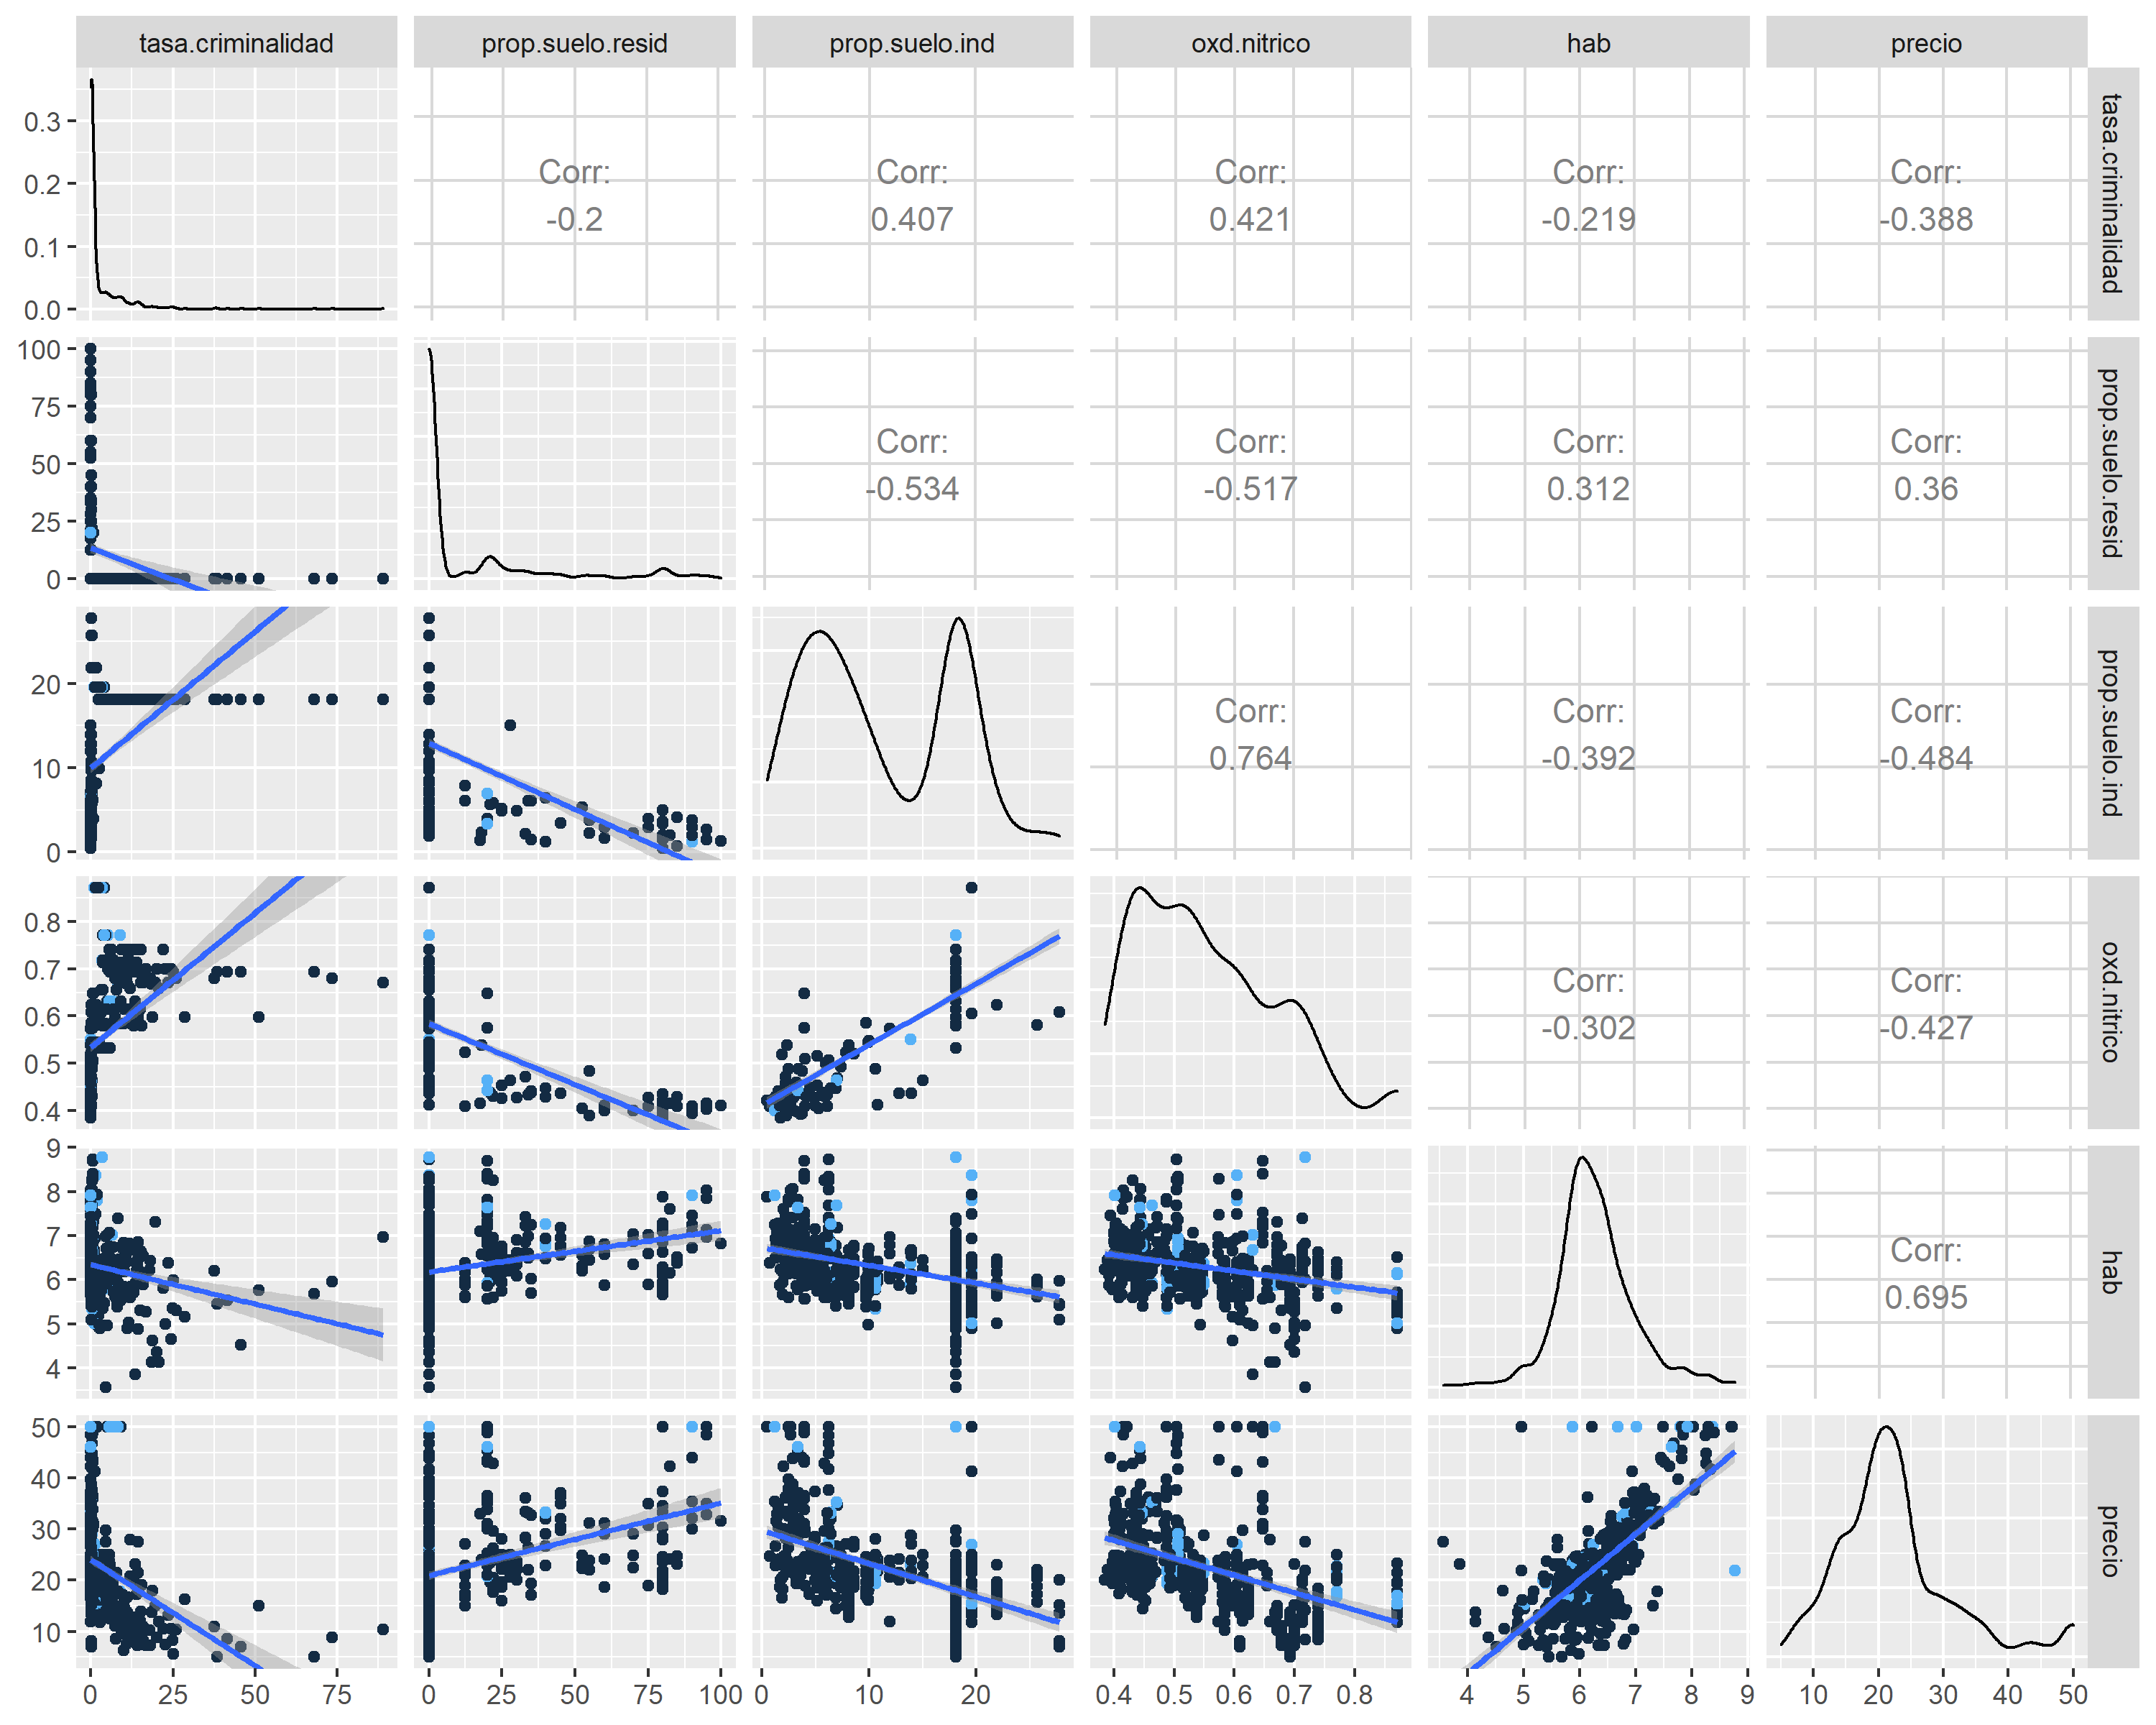
\includegraphics[scale=1]{images/pairs1-1}
	\caption[pairs]{pairs plot de las primeras 6 variables}
	\label{fig:fig3}
\end{figure}  

En el segundo conjunto de variables, resaltan la distribución de la zona de trabajo, que al contrario de lo esperado, tienen una correlación muy baja con respecto al precio, indicando poca relación lineal entre las variables. Otra variable con un comportamiento extraño, es la población de color, con un comportamiento exponencial creciente. Las variables autovías y tasa de impuesto inmobiliario están altamente correlacionadas (\textit{figura 4 [2,3]} ),por lo tanto, es importante eliminar una de las variables al estudio, debido a la colinealidad y no invertibilidad en los modelos propuestos. \\  

Para este estudio, se proponen 3 modelos, el primero es una regresión lineal con prioris independientes, este primer modelo sirve para identificar las variables que no afectan directamente al precio, después de eliminar las variables colineales y variables que no afectan al modelo se proponen 2 modelos:
\begin{itemize}
	\item Regresión lineal con prioris no independientes
	\item Red Neuronal con 1 capa, 4 neuronas y prioris independientes
\end{itemize}

Las posterioris se estimaron usando un Monte Carlo Hamiltoniano \cite{DUANE1987216} \cite{betancourt2017}, usando el algoritmo NUTS (No U turn Sampling) \cite{hoffman14a} mediante el lenguaje de programación probabilista \cite{Stan}. Para cada modelo, se realizaran 4 simulaciones de 2,000 iteraciones cada una, con un warm-up de las primeras 1000, se eligió un max\_treedepth = 11 y un adapt\_delta = 0.9

\begin{figure}[H]
	\centering
	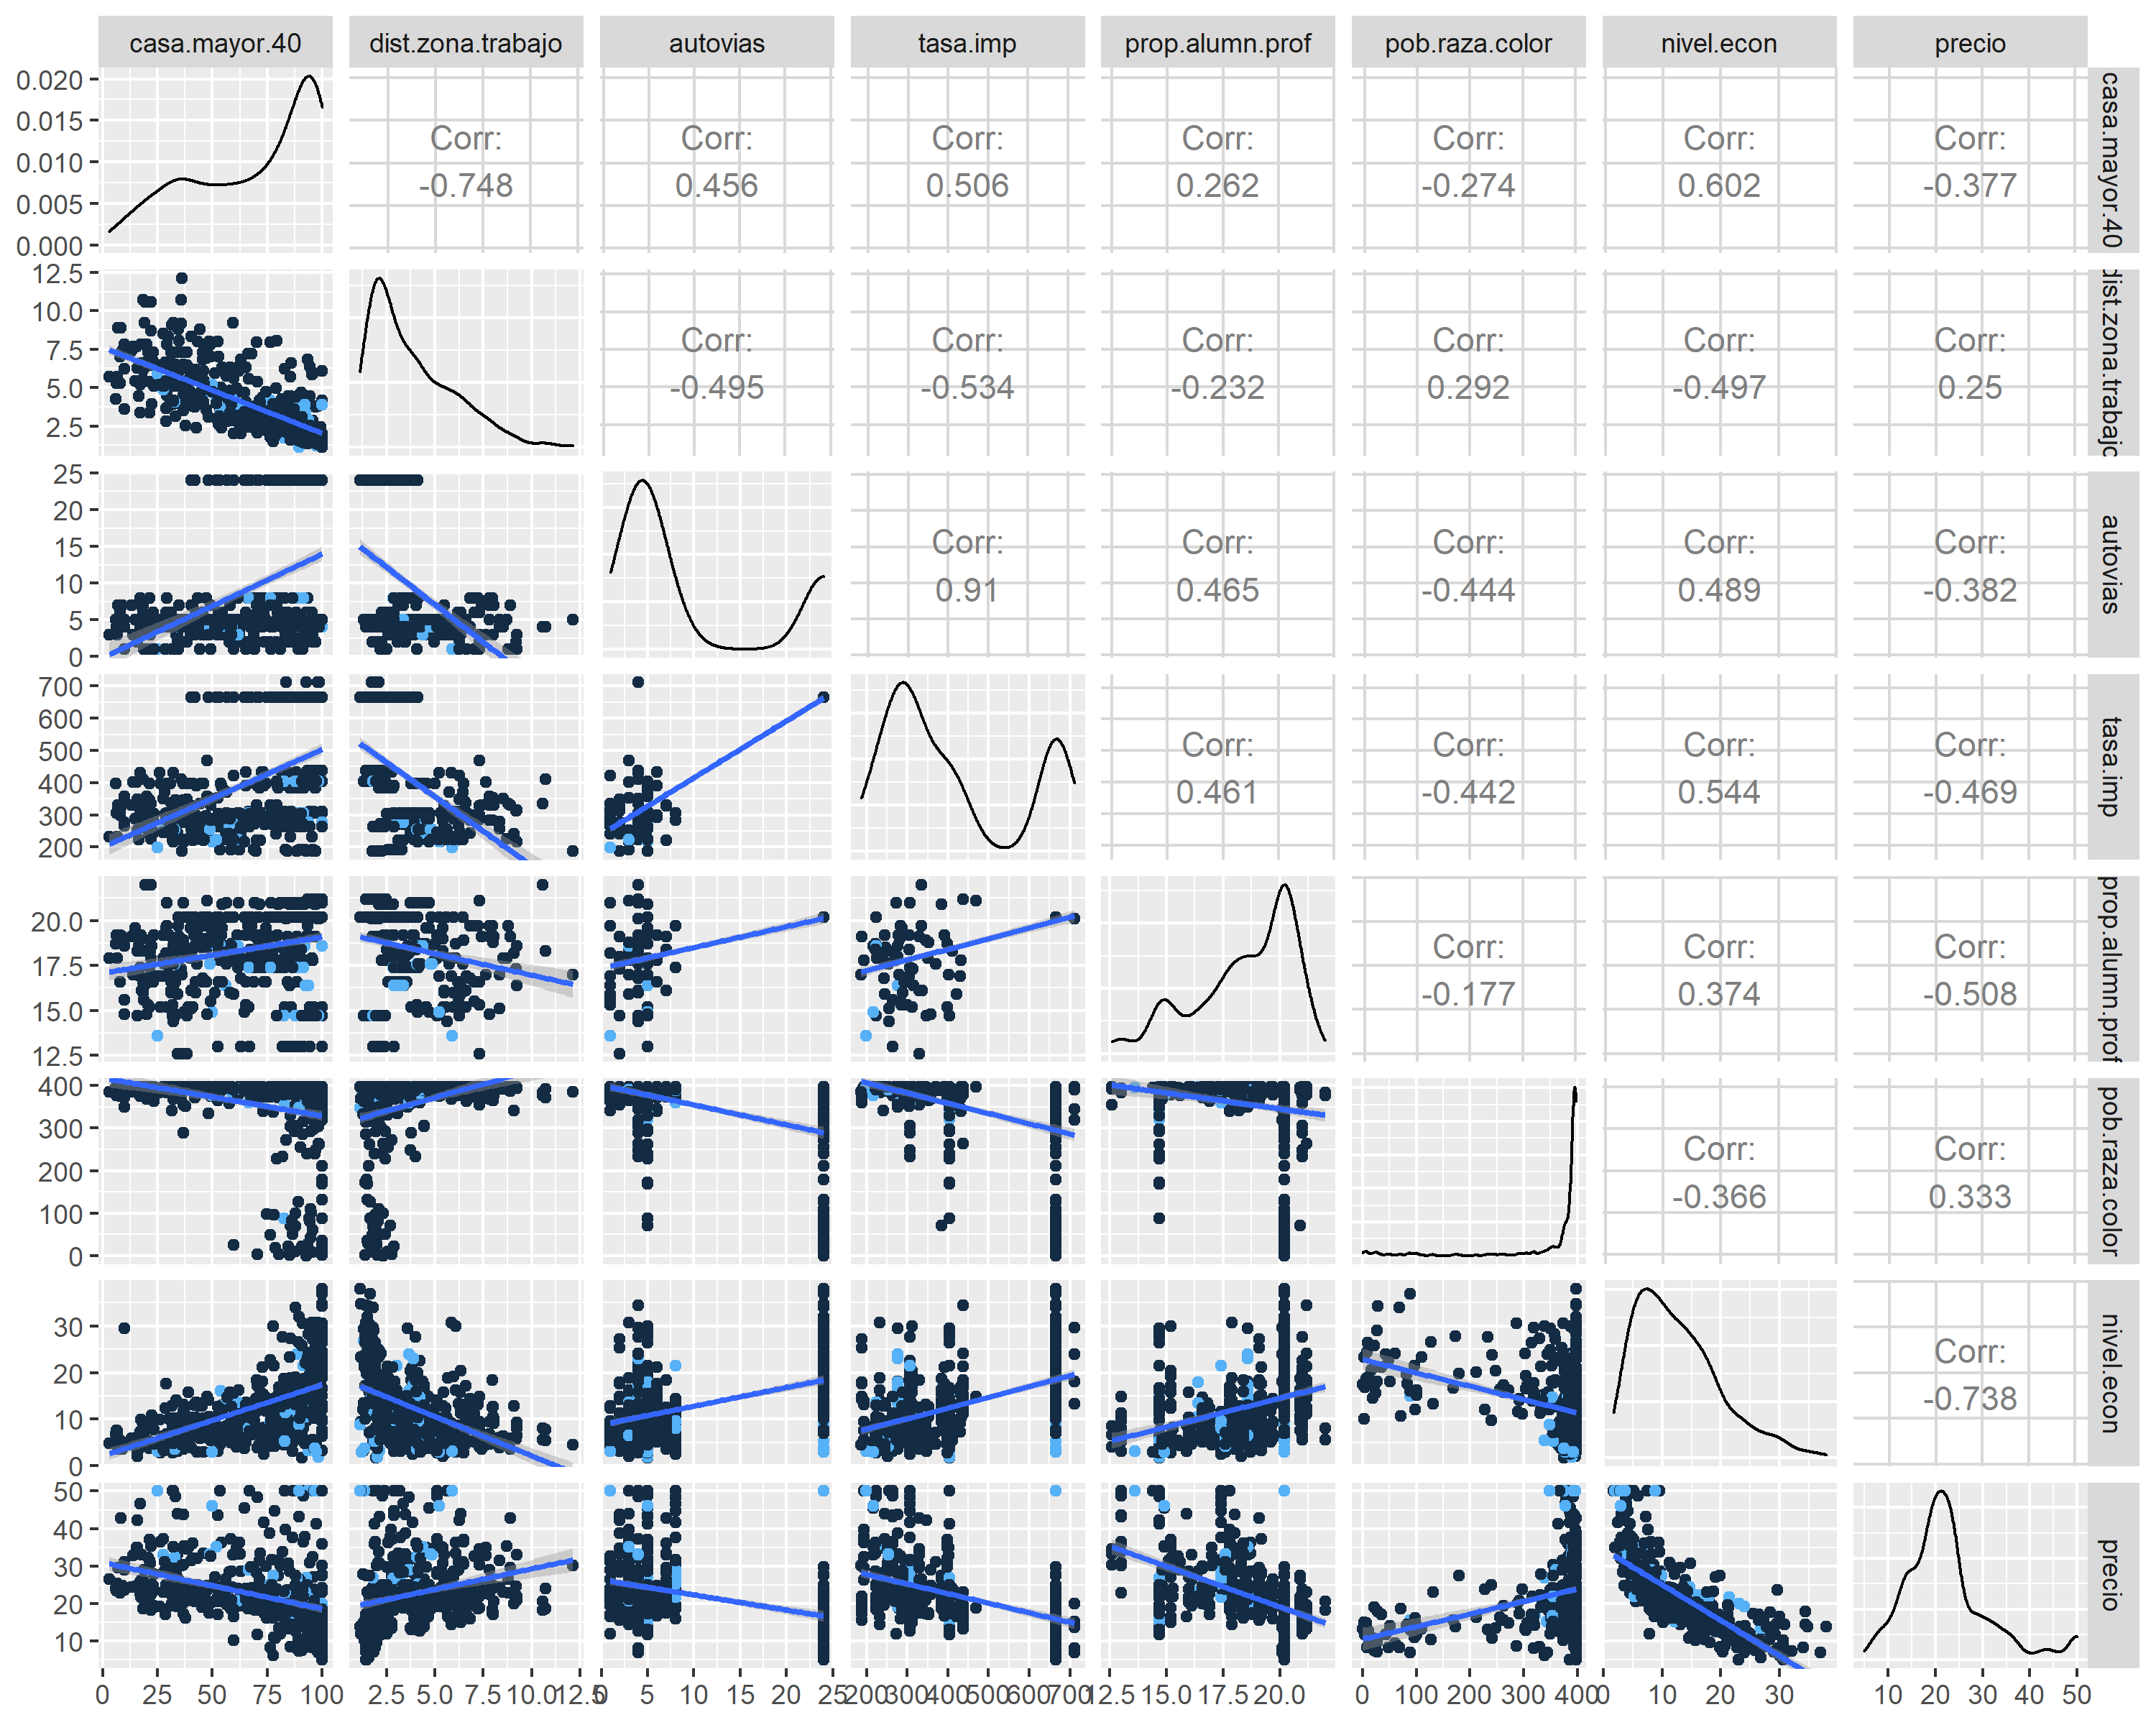
\includegraphics[scale=1]{images/pairs2-1}
	\caption[pairs]{pairs plot de las ultimas 6 variables}
	\label{fig:fig4}
\end{figure}  

\subsection{Modelo inicial: Regresion lineal Bayesiana} 
 
Este modelo es una simple regresión lineal donde cada variable explicativa afecta solamente la variable precio, se asume que la variable respuesta se distribuye normal con media y varianza desconocida, por lo tanto, el modelo es de la siguiente forma:

$$precio \sim normal(location = \alpha + \sum_{i=1}^{13}\beta_i X_i,scale =  \sigma^2)$$
$$\sigma \sim half\_student(location = 0,df = 4,scale = 5)$$ 
$$\alpha \sim student(location = 0,df = 4,scale = 5)$$ 
$$\beta_i \sim normal(location = 0,scale = 5)$$

Donde $\alpha$, $\sigma$ y las $\beta_i$ son variables desconocidas, las $X_i$ representan las 13 variables explicativas, de los datos Housing. Dado que no existe información adicional al modelo, las prioris elegidas son poco informativas que se adaptan a la geometría del espacio parametral. Al correr el modelo se obtienen los siguientes resultados:

\begin{CodeChunk}	
\begin{CodeOutput}
 		Resumen estimación de parámetros	
   variables        mean    sd    2.5\%   median   97.5\%   n_eff    Rhat
(Intercept)        36.939 5.3614  26.255  36.955  47.264  4117.100  0.9993
tasa.criminalidad -0.1122 0.0330 -0.1766 -0.1123 -0.0475  5061.617  0.9992
prop.suelo.resid   0.0467 0.0137  0.0200  0.0466  0.0744  4217.088  0.9991
prop.suelo.ind     0.0395 0.0624 -0.0845  0.0397  0.1607  3709.630  1.0006
oxd.nitrico       -17.338 3.9672 -24.917 -17.377 -9.5282  4190.938  0.9998
hab                3.8498 0.4176  3.0253  3.8420  4.6561  4156.767  0.9994
casa.mayor.40      0.0028 0.0133 -0.0234  0.0029  0.0281  4322.935  1.0007
dist.zona.trabajo -1.4823 0.2002 -1.8720 -1.4810 -1.0892  4120.718  0.9996
autovias           0.3270 0.0669  0.1974  0.3269  0.4597  2920.106  1.0002
tasa.imp          -0.0137 0.0038 -0.0211 -0.0137 -0.0063  3073.297  0.9998
prop.alumn.prof   -0.9943 0.1356 -1.2544 -0.9953 -0.7317  4579.105  0.9997
pob.raza.color     0.0097 0.0027  0.0044  0.0097  0.0152  5984.453  0.9995
nivel.econ        -0.5352 0.0502 -0.6344 -0.5350 -0.4383  4233.495  1.0006
sigma              4.7994 0.1569  4.5104  4.7931  5.1199  4826.803  1.0002
log-posterior     -1529.4 2.6582 -1535.6 -1529.1 -1525.2  1809.624  1.0010 
\end{CodeOutput}
\end{CodeChunk}

Al revisar los intervalos de credibilidad, se observan variables que no aportan nada al modelo como: las proporciones de suelo residual(2) e industrial(3), tasa de impuesto inmobiliario(9), porcentaje de casas mayores a 40 años(6), población de color(11). Estas variables no serán incluidas en los siguientes modelos.

\begin{figure}[H]
	\centering
	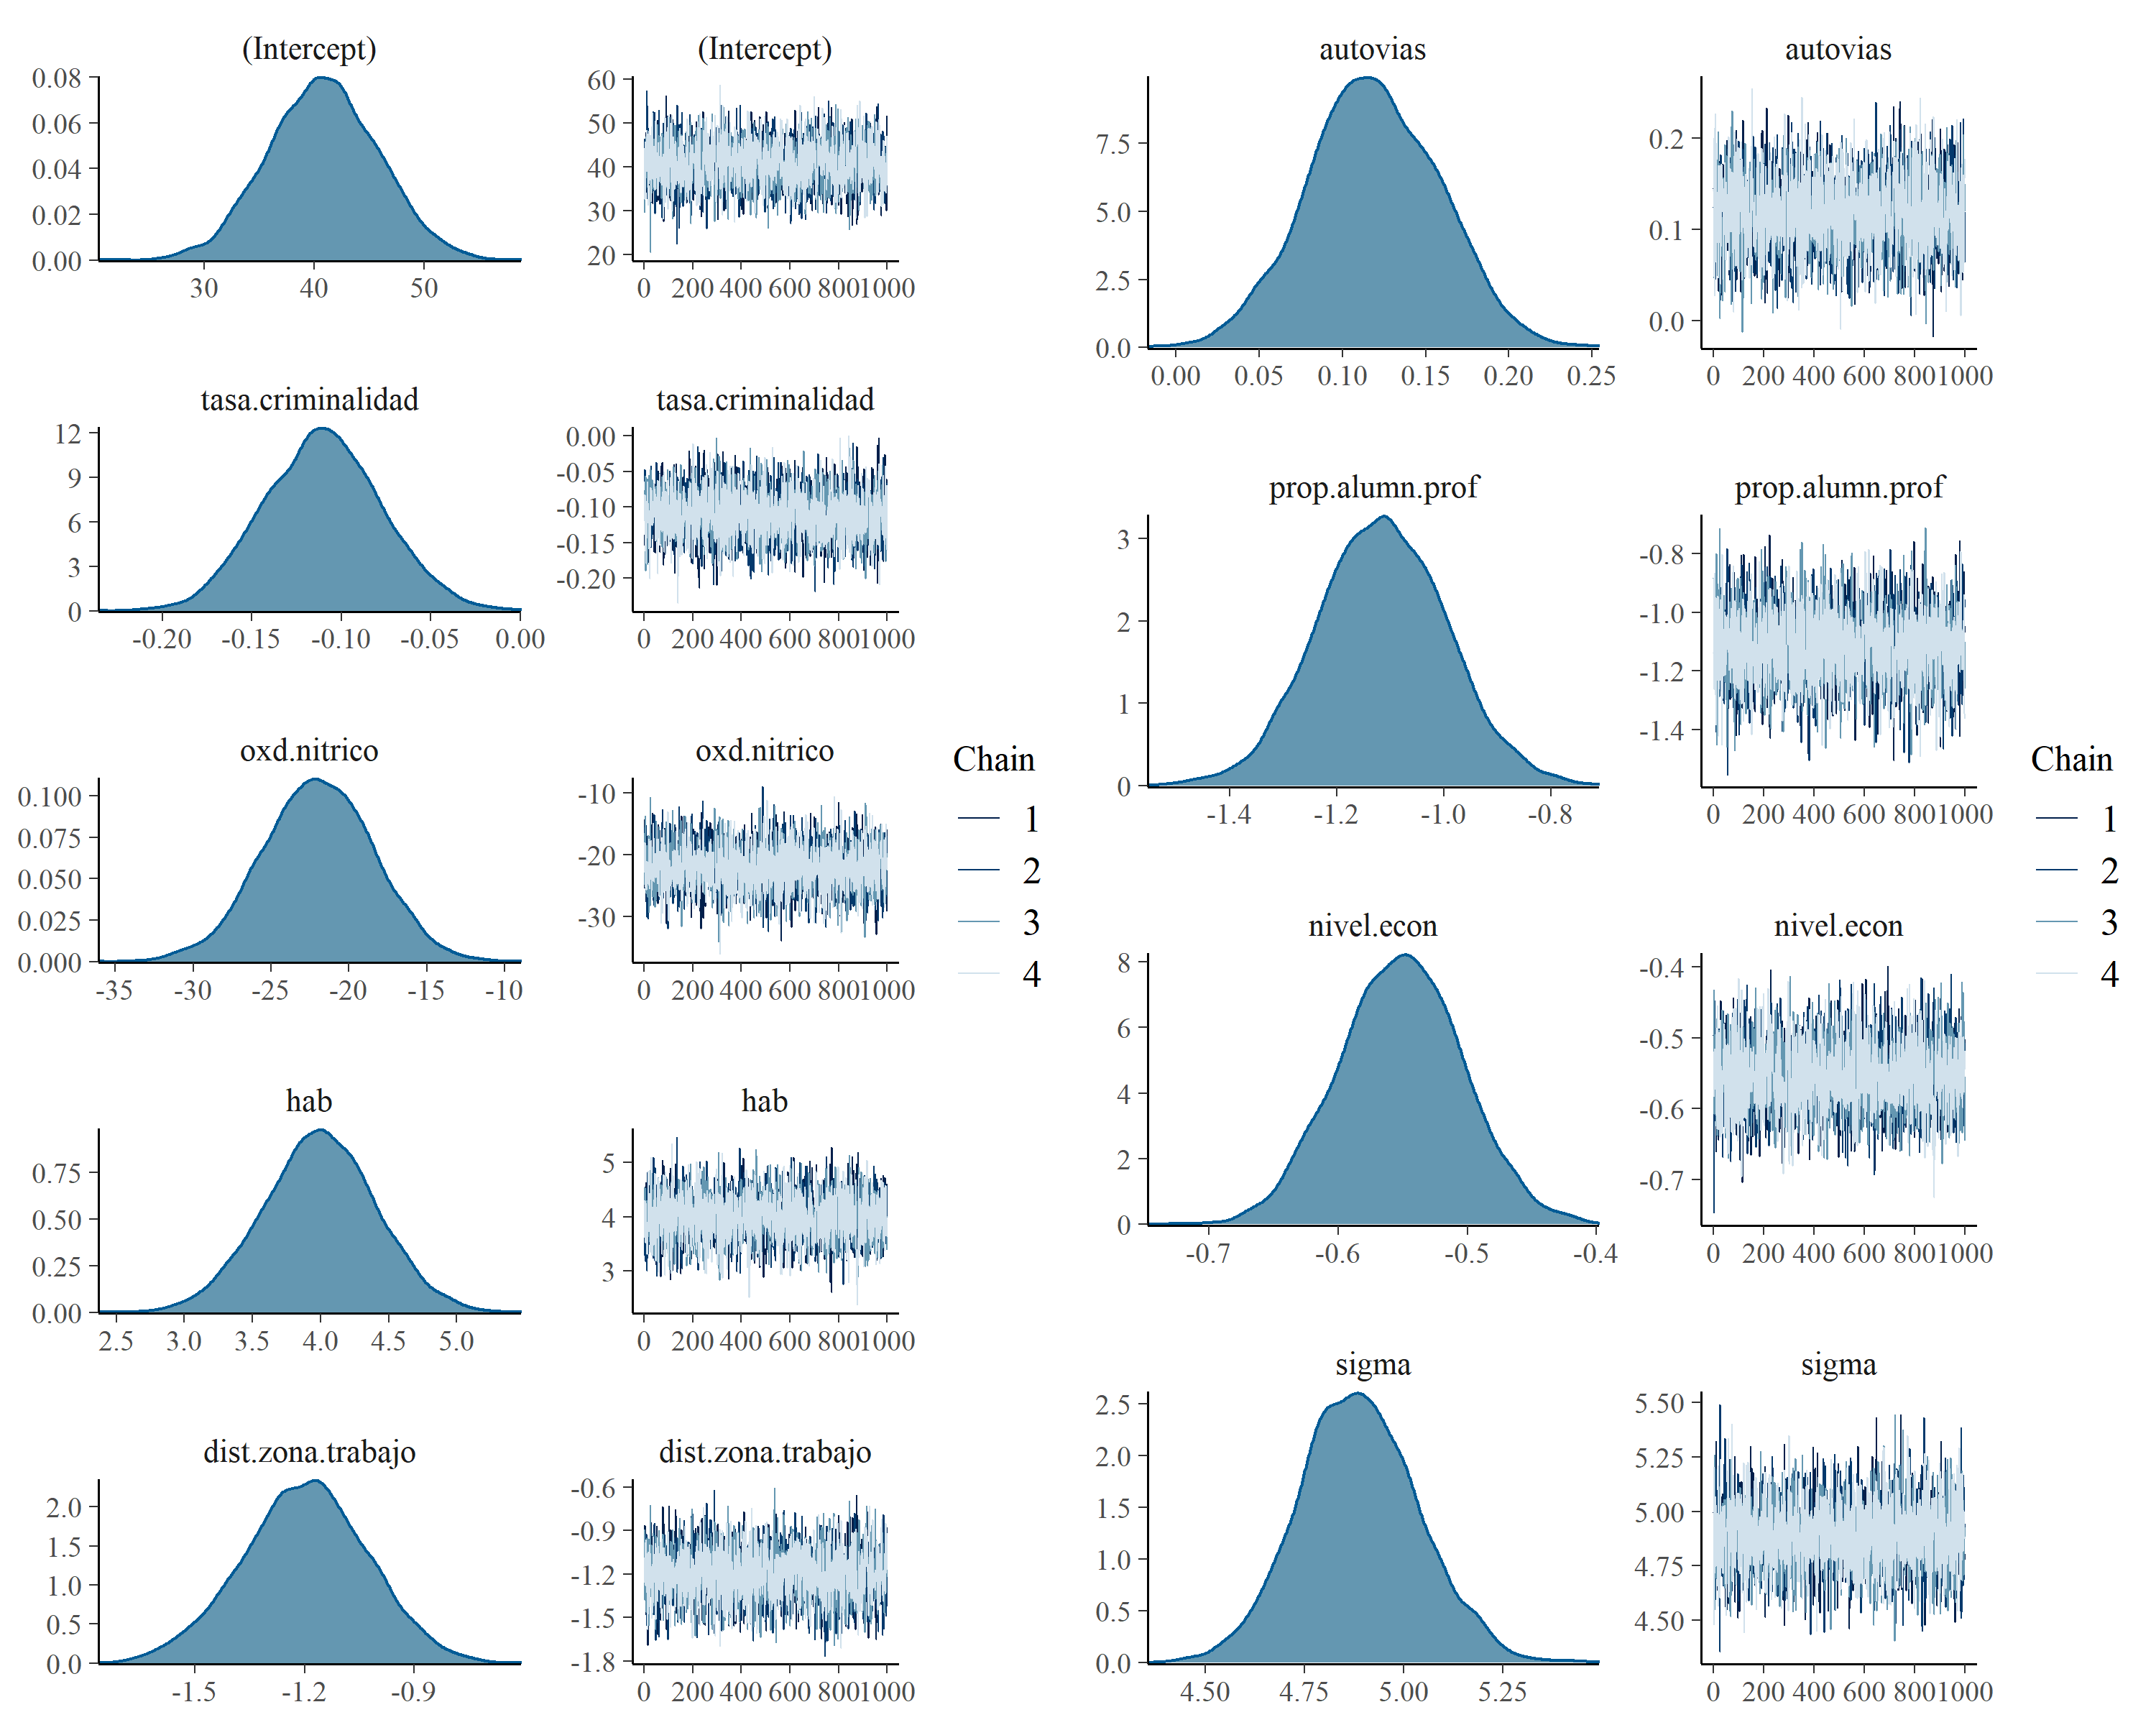
\includegraphics[scale=0.8]{images/traceplot1}
	\caption[trace1]{Gráficos de densidad y traceplots de coeficientes en modelo 1}
	\label{fig:fig5}
\end{figure}

Se procede a realizar un diagnostico de los parámetros ajustados, el potencial de convergencia $\widehat{R}$ es cercano a 1, indicando que las cadenas convergen,  el menor tamaño de muestra efectivo (\textit{n\_eff}) es mayor a 1,809 observaciones, eso indica que las 4 muestras simuladas de cada parámetro representan al menos 1,800 observaciones de ensayos independientes, en la \textit{figura 5}, las 4 cadenas simuladas en cada uno de los parámetros convergen al mismo punto y son estacionarias indicando que no existen problemas de convergencia. Finalmente, los density plots de las distribuciones posterioris son unimodales, por lo tanto, la media a posteriori es un estimador óptimo en cada uno de los parámetros.\\

Con este modelo se han eliminado 6 variables que no contribuyen al precio de venta de las casas, en las siguientes secciones se presenta una comparación entre una red neuronal Bayesiana y un regresión lineal con prioris dependientes.\\

\begin{figure}[H]
	\centering
	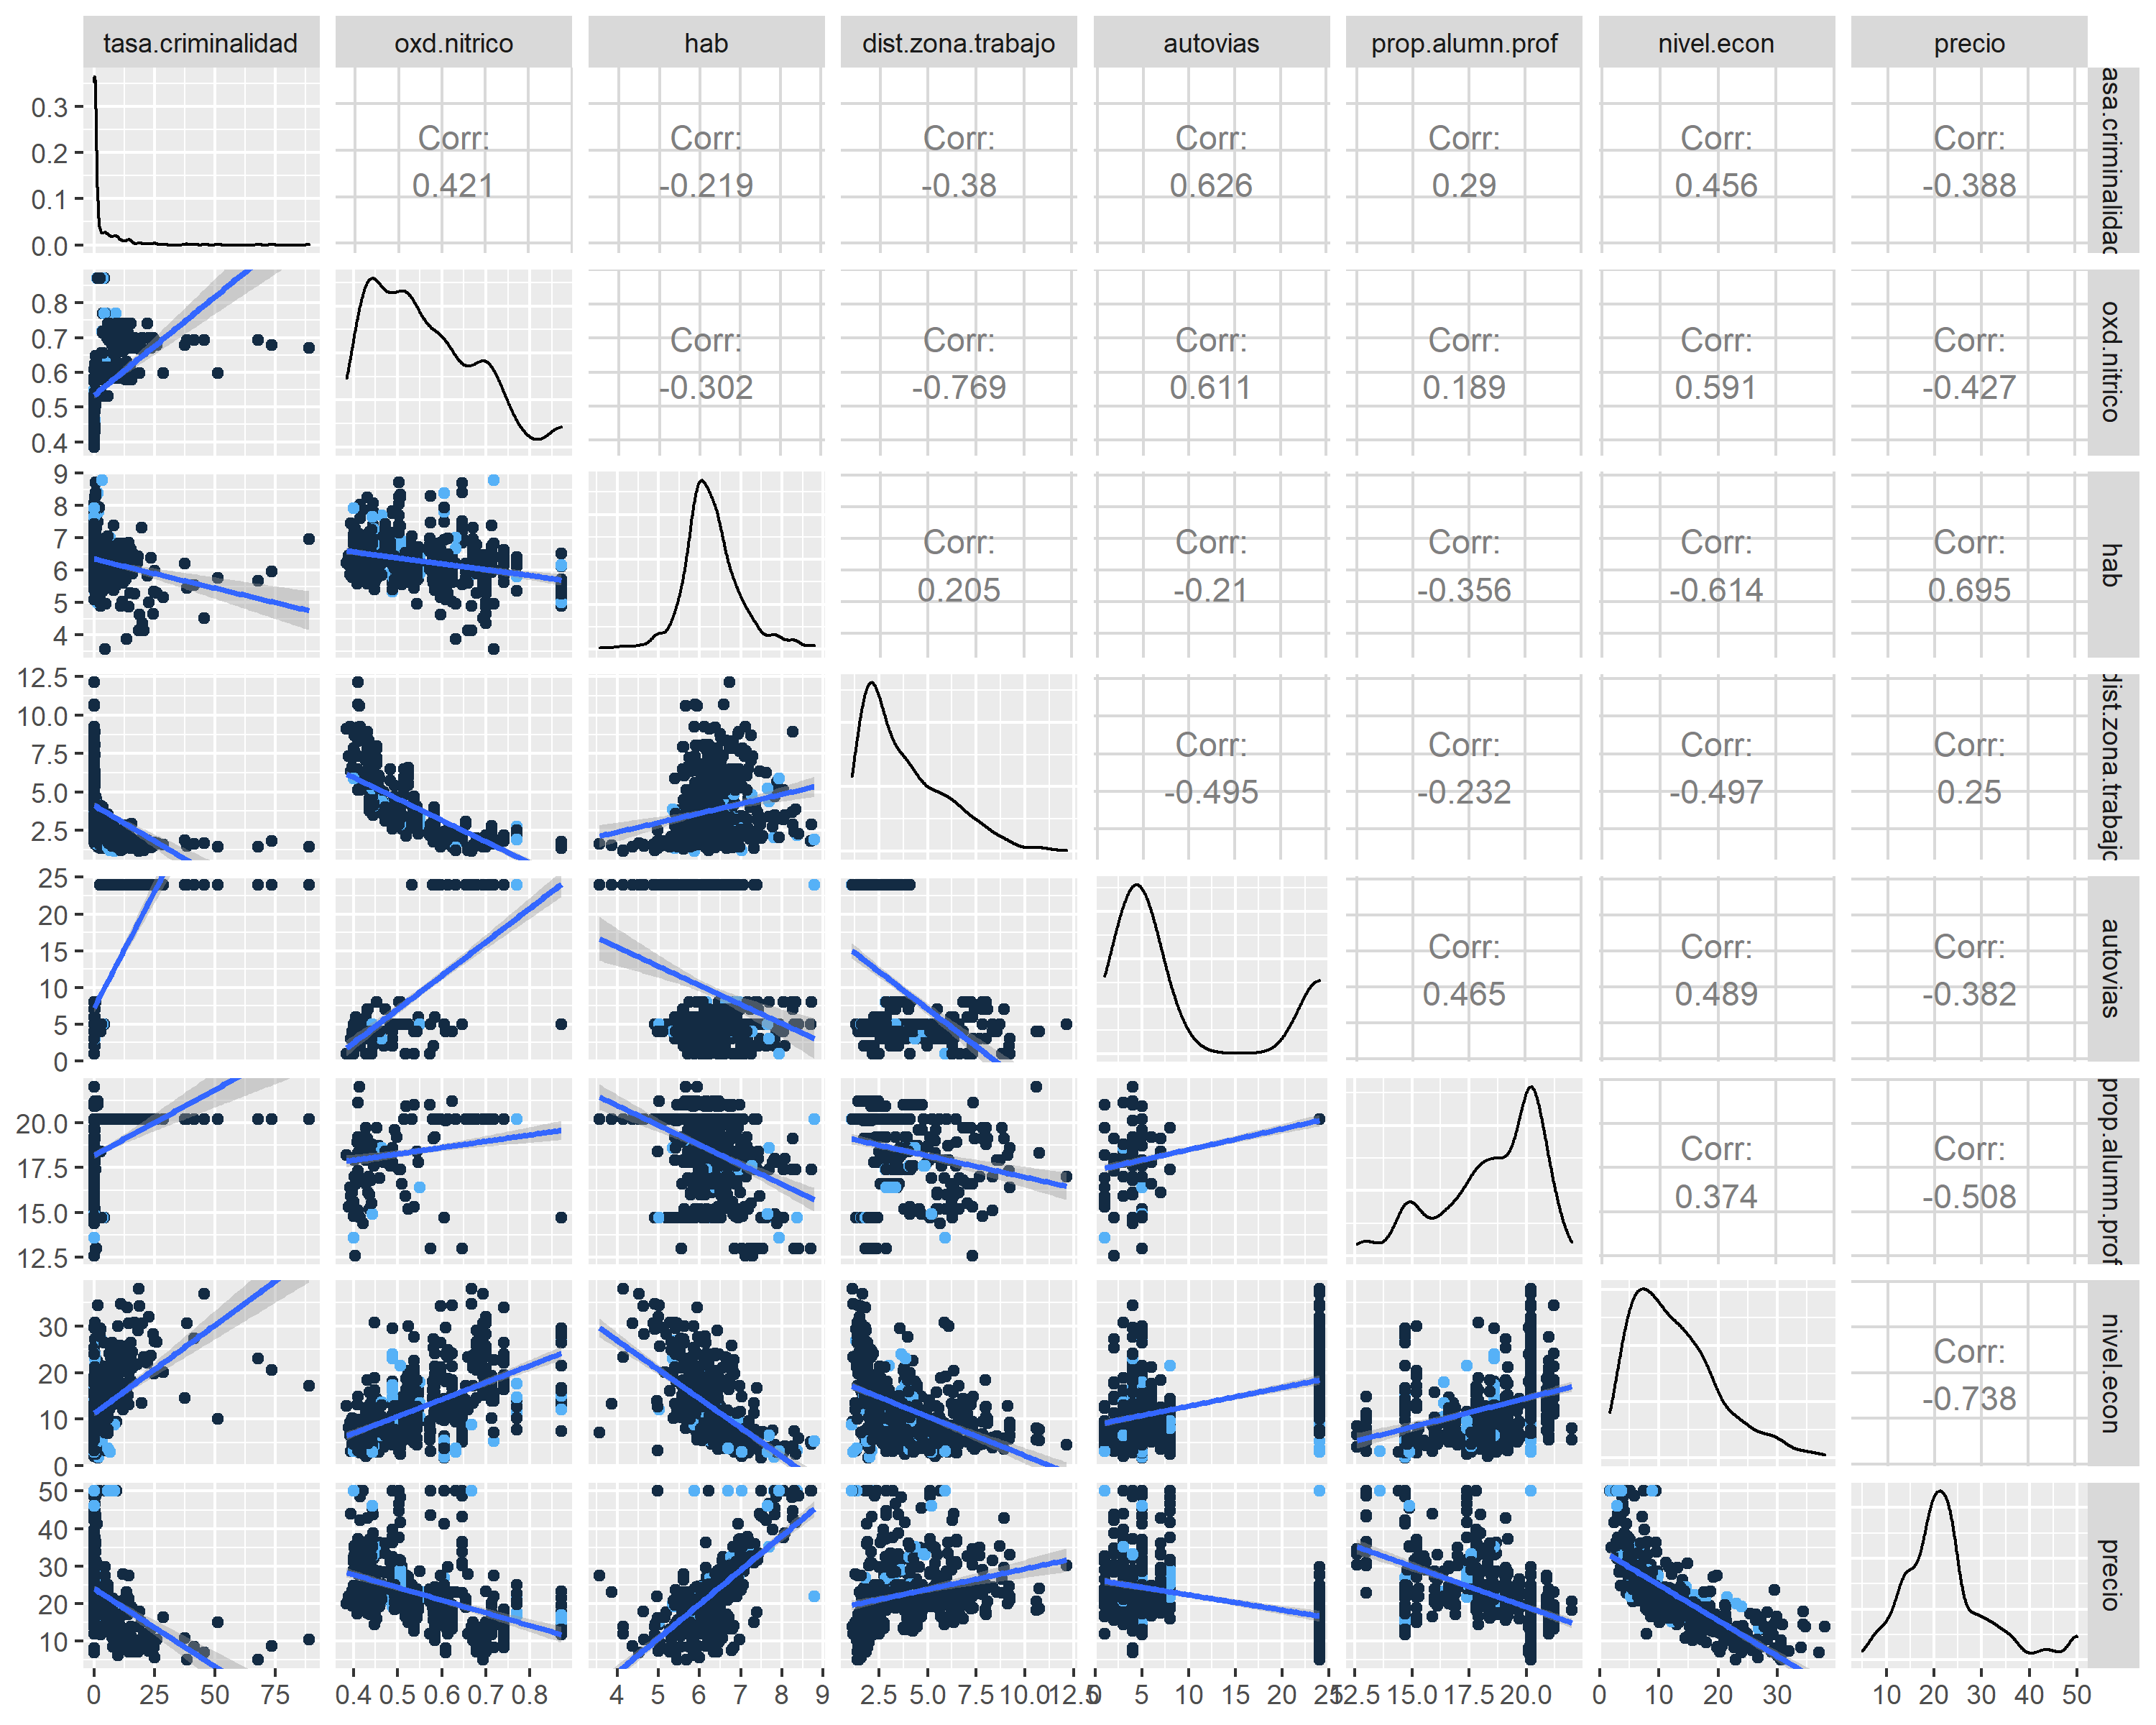
\includegraphics[scale=1]{images/pairs3-1}
	\caption[pairs]{pairs plot de las 8 variables que contribuyen linealmente al precio de ventas}
	\label{fig:fig6}
\end{figure}

\subsection{Regresi\'on lineal Bayesiana prioris dependientes}

Los datos en la \textit{figura 6} muestran que las variables explicativas son no correlacionadas entre si. Por ejemplo, el porcentaje de oxido nítrico y la distribución de la zona de trabajo parecen tener una relación polinómica. Por lo tanto, el supuesto de independencia entre los parámetros es una suposición muy restrictiva, para evitar dichas restricciones se propone el siguiente modelo:
$$ precio \sim normal(location = \beta_0+ \sum_{i=1}^{8}\beta_i X_i,scale =  \sigma^2)$$
$$Intercept \sim student(location = 0,df = 4,scale =1)$$
$$sigma \sim half\_cuachy(location = 0,scale =5)$$
$$\beta = (\beta_1,...,\beta_{8})$$ 
La distribución a priori propuesta para $\beta$ es una normal multivariada,
$$\beta \sim Normal_8(location = 0,scale = \Sigma)$$
Ahora bien, la matriz de covarianza $\Sigma \in \mathbb{R}^{8}$ se asume no diagonal, y se factoriza de la siguiente forma:
$$\Sigma = D^t\Omega D$$
Donde  $D = diag(\lambda_1,\lambda_2,...,\lambda_{8})$ es una matriz diagonal de desviaciones estándar y $\Omega$ es la matriz de correlaciones. Las distribuciones a  priori elegidas para D y $\Omega$ son:

$$\lambda_i \sim cauchy(location = 0,scale = 4)$$ 
$$\Omega \sim LKJ(df = 2)$$

Donde LKJ es una distribución matricial propuesta por \cite{LKJ2009}. Esta generaliza la distribución beta, y su forma es una variedad concava en el hiper-cubo $[0,1]^8$.


\begin{figure}[H]
	\centering
	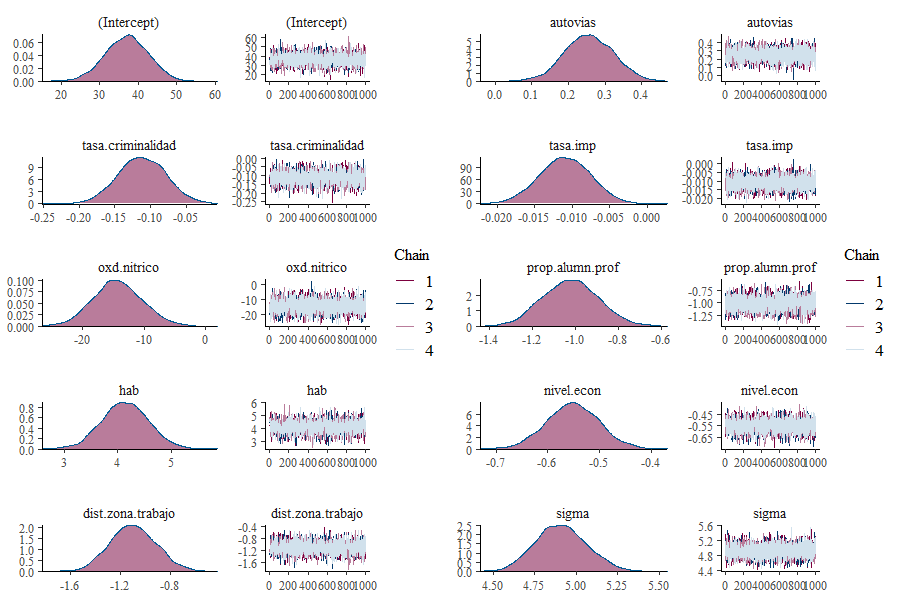
\includegraphics[scale=0.8]{images/traceplot2}
	\caption[trace1]{Gráficos de densidad y traceplots de coeficientes en modelo 1}
	\label{fig:fig7}
\end{figure}

Todos los parámetros de esto modelo convergen, con tamaños de muestra efectivos aceptables (no muy bajos), las distribuciones a posteriori no son multimodales, por lo tanto, el modelo es identificable, este modelo, tubo un alto costo computacional, en comparación al modelo inicial con prioris independientes. 

\begin{CodeChunk}	
\begin{CodeOutput}
	                Resumen estimación de parámetros
variables            mean  sd     2.5\%  median   97.5\%   n_eff    Rhat
(Intercept)        37.351 5.448  26.585  37.386  47.930 1832.535  1.0006
tasa.criminalidad -0.1119 0.034 -0.1790 -0.1121 -0.0445 4010.858  0.9999
oxd.nitrico       -14.430 4.002 -22.196 -14.553 -6.4797 2324.414  1.0005
hab                4.1197 0.435  3.2785  4.1153  4.9906 2371.859  1.0000
dist.zona.trabajo -1.1035 0.184 -1.4624 -1.1041 -0.7374 3027.111  1.0005
autovias           0.2582 0.067  0.1231  0.2580  0.3917 2696.030  0.9997
tasa.imp          -0.0110 0.003 -0.0178 -0.0111 -0.0041 3528.300  0.9996
prop.alumn.prof   -1.0280 0.128 -1.2817 -1.0308 -0.7730 2831.665  1.0002
nivel.econ        -0.5521 0.051 -0.6531 -0.5534 -0.4495 3367.700  0.9997
sigma              4.9111 0.158  4.6154  4.9052  5.2395 5360.408  1.0003
log-posterior     -1567.9 5.219 -1579.2 -1567.6 -1559.0 1668.808  1.0017 
\end{CodeOutput}
\end{CodeChunk}

\subsection{Red Neuronal una capa y 4 neuronas}

Este modelo acepta una representación para $f$ de forma no recursiva mediante la siguiente ecuación:

$$f(X) = \beta_0 + \sum_{k=1}^h v_k tanh\left(a_k + \sum_{j=1}^d \beta_{kj}X_j \right)$$

Donde $h=4$ son el número de neuronas en la primera capa, y $d = 8$ son el número de variables predictivas utilizadas, se asume independencia entre las distribuciones a priori de los parámetros. Por lo tanto, el modelo es:

$$Y_i \sim normal(location = f(X_i),scale = sigma^2)$$
$$sigma \sim half\_cuachy(location = 0,scale = 1)$$
$$\beta_0 \sim student(location = 0,df= 4,scale = 1)$$
$$a_j \sim student(location = 0,df=4,scale = 1)$$
$$\beta_{jk} \sim normal(location = 0,scale = 1)$$

Para $i = 1,2,\ldots,n$, $k = 1,2,3,4$ y $j = 1,2,\ldots,8$. Debido a la alta cantidad de parámetros, solo se presentan las importancias de la primera capa ($v_k$), la escala del modelo ($\sigma$). A diferencia de los modelos anteriores, las cadenas convergen en diferentes puntos que representan los óptimos locales de la red, en la \textit{figura 8} se observa que las distribuciones a posteriori son multimodales, por lo tanto, el modelo es no identificable, y la inferencia de los parámetros no brindan buenas aproximaciones. 

\begin{CodeChunk}	
\begin{CodeOutput}
 		Resumen estimación de parámetros
  variable       mean   sd    2.5\%   50\%  97.5\% n_eff    Rhat
 (Intercept)    10.89  1.022  9.329  11.08  12.09  1418    2.001  
 Neurona[1]    -18.07  18.36 -41.51 -19.80 -8.312  33.60   2.010
 Neurona[2]     74.17  75.69 -0.023  51.85  193.0  37.66   2.009
 Neurona[3]    -8.808  39.79 -79.58  0.038  37.98  29.12   2.017  
 Neurona[4]     2.169  10.61 -11.97  2.547  15.56  12765   2.001 
 sigma          0.007  0.004  0.002  0.008  0.012  13.47   2.061 
 log-posterior 1869.4  211.5  305.1 1607.5 2395.7  12.398  2.080  
\end{CodeOutput}  
\end{CodeChunk}


\cite{Paige2001} proponen usar una priori t de student multivariada jerárquica, para resolver el problema de identificabilidad. Para definir una priori multivariada de forma jerárquica se realiza de la siguiente forma:

$$X \sim N_v(0_v,D^t\Sigma D)$$
$$\Sigma  \sim Wishart(I)$$
$$D = diag(\lambda_i,\ldots,\lambda_i)$$
$$\lambda_i \sim inv\_gamma(v/2,v/2)$$
$$v \sim gamma(4,0.1)$$

Dicho algoritmo no fue implementado debido al alto costo computacional.


\begin{figure}[H]
	\centering
	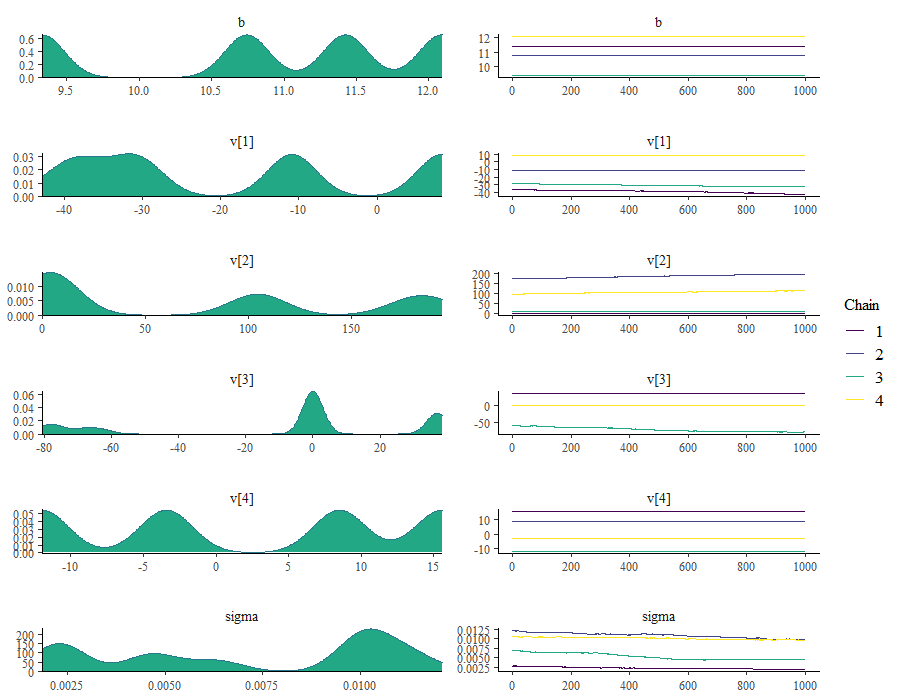
\includegraphics[scale=0.8]{images/traceplot3}
	\caption[trace3]{Gráficos de densidad y traceplots de coeficientes en modelo 3}
	\label{fig:fig8}
\end{figure}


\section{Comparación de los modelos y conclusiones}

Para comparar ambos modelos se proponen los criterios de la log verosimilitud (log-lik), el ajuste del modelo mediante, los residuos, mean square error (MSE) y su raíz (RMSE), el mean absolute error (MAE), el criterio de \cite{watanabe} (WAIC) , que es una generalización propia y más eficiente de los criterios AIC y DIC,  y un leave one out cross validation (loo) \cite{loo}.  Se descarta el factor de Bayes \cite{bayesfactor}, debido a que computar la predictiva de la red neuronal es computacionalmente costoso.\\

\begin{table}[h]
\centering
\begin{tabular}{lcccc|cccc}	
          & \multicolumn{4}{c}{Red Neuronal} & \multicolumn{4}{c}{Regresión lineal}\\ 
\hline
Indicador & 2.5\% & media & mediana & 97.5\% & 2.5\% & media & mediana & 97.5\%  \\  
\hline
MSE       & 7.31e-6  & 1.08e-4 & 1.09e-4 & 2.47e-4 & 42.33 & 48.18  & 48.09  & 54.57\\ 
RMSE      & 2.7e-3   & 9.35e-3 & 1.04e-2 & 1.57e-2 & 6.506 & 6.938  & 6.935  & 7.387\\ 
MAE       & 2.09e-3  & 7.31e-3 & 8.10e-3 & 1.24e.2 & 4.988 & 5.347  & 5.343  & 5.714\\ 
residuals & -6.9e-3  & -3.7e-6 & 4.3e-4  & 5.98e-3 & -6.61 & 4.1e-3 & -0.778 & 11.79\\ 
loglik    & -2,461   &  -1,933 & -1,797  & -1,584  & -1,518& -1,523 & -1,522 & -1,529\\ 
WAIC      & -3,504   & -3,428  & -       & -3,352  & -3,129& -3,064 & -      & -2,999\\
looic     & -3,569   & -3,509  & -       & -3,449  & -3,129& -3,064 & -      & -2,999\\
\hline
\end{tabular}
\caption{Comparación de modelos} 
\label{tab:tab1}
\end{table}

En la tabla anterior se presentan las medidas a posteriori de cada uno de los indicadores, como la media, mediana  e intervalos de credibilidad al 95\%. Además, los valores del WAIC y loo coinciden debido a que el WAIC converge asintóticamente al loo \cite{vehtari}. La red Neuronal ofrece un peor ajuste a los datos que el modelo lineal (\textit{ver loglik,WAIC y loo}), además, su complejidad e identificabilidad hacen que el modelo no sea útil para explicar los datos. Pero ofrece mejores predicciones que la regresión lineal (\textit{ver MSE, RMSE,MAE y residuos}), por lo tanto, las redes no deben ser descartadas a priori y ofrecen una buena alternativa cuando la tarea a realizar sea predecir solamente.

\bibliography{refs}


\end{document}
